% PARTIE 2 - TECHNIQUE %%%%%%%%%%%
% CHAPITRE 3 %%%%%%%%%%%%%%%%%%%%%
%%%%%%%%%%%%%%%%%%%%%%%%%%%%%%%%%%
Pour développer une carte Web, il ne suffit pas d'avoir des données structurées dans une base de données, il est également nécessaire de concevoir leur agencement et leur visualisation\footcite{LAGNELManuel2021, ANDRYChapitre2022, CEJUDObreve2022}. Ce troisième chapitre introduit une nouvelle étape de conception de la carte qui consiste à définir des objectifs de développement spécifiques à la cartographie Web. Dans un premier temps, ces objectifs sont établis en comparant divers éléments de cartes Web issues de projets de recherche. Après cette présentation de l'état de l'art, il s'agit de hiérarchiser les priorités de développement à l'aide de plusieurs méthodes. Enfin, une analyse du contenu de la base de données est intégrée à ce processus : il apparaît en effet primordial de bien comprendre le contenu avant de l'intégrer dans l'application pour le développement de la carte. Cette analyse quantitative permettra d'anticiper les possibles biais de représentation qui pourraient survenir lors de la visualisation.

%%%%%%%%%%%%%%%%%%%%%%%%%%%%%%%%%%%%%
% SECTION %%%%%%%%%%%%%%%%%%%%%%%%%%%
\section{État de l'art de la visualisation cartographique des données sur le Web}\label{section:choix-carto}
Cette première section offre un aperçu non exhaustif de l'état de l'art des visualisations cartographiques des données sur le Web. En couvrant à la fois la réflexion théorique et la mise en œuvre technique, seront listés et comparés des éléments cartographiques de projets de recherche, en particulier en histoire de l'art. Ce tour d'horizon sert à donner quelques repères et points de référence pour définir au mieux les fonctionnalités à privilégier et celles à mettre de côté pour la visualisation de données géohistoriques du projet Richelieu.

\subsection{En théorie : l'image est une écriture}
Rappelons-le, la visualisation est une \enquote{présentation visuelle sur un écran, sous \textit{forme d'image} alphanumérique ou graphique, d'un ensemble d'informations traitées par des moyens informatiques} (Larousse). Pourquoi le projet Richelieu favorise-t-il l’utilisation de l’image plutôt que de celle de l'écriture pour explorer et étudier le quartier~?  Dans les sciences humaines et sociales, l'écriture demeure la forme conventionnelle de l'expression scientifique. En histoire de l'art, cette tradition est d'autant plus marquée que l'écriture sert à décrire et à interpréter les œuvres. Dans ce cas, l'image est ainsi secondaire à l'écriture. Toutefois, il est reconnu que les enluminures, gravures, peintures, photographies et autres représentations graphiques sur une surface plane servent tout autant à exprimer un propos\footcite{GRANDJEANIntroduction2015}. L'image est un moyen d'expression visuelle. La visualisation des données s'introduit dans cette chronologie des traditions narratives. L’écriture est également une expression mais par son système de signes conventionnels, il s'agit d'un moyen écrit. Les deux fournissent un effort d’abstraction pour rendre le sensible, le réel et le matériel visible. Toutefois, l’image permet d'atteindre un niveau d'abstraction que l'écriture ne peut pas toujours atteindre, offrant une échelle de représentation différente et souvent plus immédiate pour visualiser le réel\footcite{CHRISTINLecriture2020}. Il est par exemple plus simple de représenter le globe terrestre par une image que par un texte. 

Même si un proverbe dit qu'\enquote{une image vaut mieux que mille mots}\footnote{Ce proverbe est attribué à Confucius.} elle ne peut se réduire à elle-même dans le domaine scientifique. Cela ne signifie pas pour autant qu'elle soit nécessairement accompagnée d'un texte écrit sinon de connaître la démarche dans laquelle la visualisation a été réalisée. Cette idée est principalement développée par l'historien contemporanéiste et spécialiste des humanités numériques, Martin Grandjean, qui estime qu'\enquote{il faut distinguer les visualisations qui \textit{découlent} d’un savoir scientifique et les visualisations qui \textit{créent} un savoir scientifique}.\footcite{GRANDJEANIntroduction2015} En d'autres termes, il définit deux objectifs de visualisation : celle à des fins de \textit{démonstration} d'un savoir déjà établi et celle qui sert à la \textit{recherche} pour constituer un nouveau savoir. Cette distinction fondamentale clarifie l'objectif de la démarche visuelle. En effet, dans le premier cas, les visualisations sont utiles pour rendre un savoir accessible et compréhensible, à des fins pédagogiques par exemple. Tandis que le second cas a pour but d'explorer des données complexes révélant des questions nouvelles voire des perspectives de recherches inattendues. Il affirme par ailleurs que ce dernier cas n'est pas destiné à être publié. 
\begin{figure}[ht!]
    \centering
    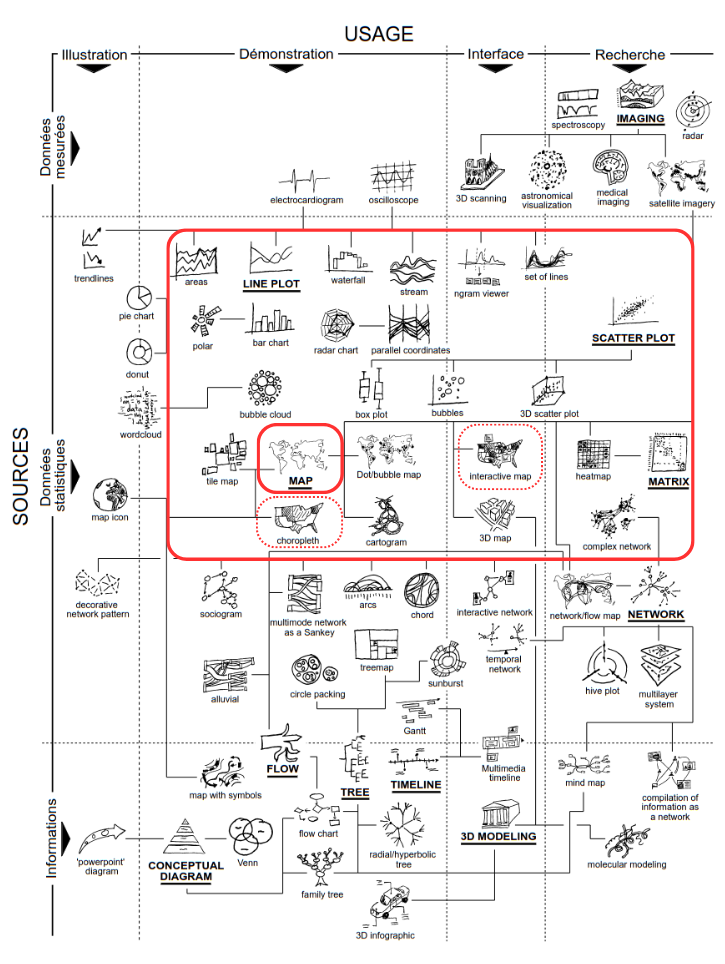
\includegraphics[width=1\linewidth]{images/typologie_dataviz.png}
    \caption{Typologie de la visualisation de données selon deux axes : le type de sources
utilisées (vertical) et le type d’usage (horizontal), Grandjean, 2022.}
    \label{fig:typologie_dataviz}
\end{figure} 

Qu'en est-il du projet Richelieu ? La visualisation des données telle qu'elle a été définie par le projet correspond aux deux cas. Certains axes de recherche sont confirmés et rédigés au sein d'articles scientifiques. Dans ce cas, la carte est une démonstration de ce qui est déjà prouvé, dit et connu. Mais la carte est aussi attendue comme outil de recherche à travers laquelle des hypothèses sauraient se formuler. Surtout, la carte a pour but d'être publiée et à destination d'un large public, aussi bien expert que novice. Ce caractère ambivalent de la carte créé une ambiguïté qui est également établie par l'auteur mais au sein d'une autre de ses publications\footcite{GRANDJEANvisualisation2022} dans laquelle il dresse une classification des typologies de visualisations de données. Parmi ce large panorama, la carte offre un caractère ambivalent oscillant entre visualisation de \enquote{démonstration} et de \enquote{recherche}. 

Il existe de nombreuses classifications des typologies de visualisations de données\footnote{Parmi les plus connues : le \href{https://github.com/Financial-Times/chart-doctor/blob/main/visual-vocabulary/poster.png}{Visual Vocabulary} du Financial Time, les catalogues \href{https://datavizcatalogue.com/FR/}{Data Visualization Catalog}, le \href{https://datavizproject.com/}{Data Viz Project} et le \href{https://flowingdata.com/chart-types/}{Flowingdata}. Cliquer sur le nom des typologies pour accéder aux sites Web.}  mais celle que Grandjean propose est intéressante à plusieurs titres (\ref{fig:typologie_dataviz}). Tout d'abord, sa classification est une aide réelle avant la mise en production d'une visualisation. En fonction des types de sources utilisées et des types d'usage définis, une forme de visualisation peut se distinguer. 

Pour le projet Richelieu, les sources sont des données extraites, en opposition aux informations généralistes, ce qui réduit considérablement le type de visualisations. Un \acrshort{uuid} n'est pas comparable au schéma numérique de la \acrshort{bnf} par exemple. Il ne s'agit pas en effet d'une infographie qui repose sur la compilation d'informations impliquant une approche plus \enquote{manuelle} mais bien d'une visualisation pour laquelle les données sont \enquote{automatiquement} captées par un outil informatique dont le résultat est parfois plus difficilement contrôlable. Ensuite, nous savons que la visualisation du projet a pour objectif d'être utilisée comme une interface, et, selon le graphe, elle est à l'intersection de la démonstration et de la recherche. Enfin, parmi les grandes familles de typologies de visualisations, telles que le nuage de points, le réseau ou le graphique en ligne ou en barre, la carte s'impose pour le projet Richelieu - notamment en raison du caractère spatial des données. Selon la définition de Grandjean, la carte se décline alors  en de nombreuses autres typologies secondaires, parmi lesquelles deux se démarquent : la carte choroplèthe et la carte interactive. La première proposition organise la donnée par zone, nos lieux symbolisés par les polygones, qui respecte la réalité géographique et est structurée en variable de données. Cela permet ainsi de visualiser les variations de données d'une zone à une autre, souvent signifiées par la couleur. La seconde carte est plus évidente puisque c'est une interface qui permet d'accéder aux données et d'interagir avec elles, et que le projet utilise les langages du Web interactif, dont le JavaScript dans Vue.js. La carte du projet Richelieu serait donc une association de ces deux typologies. Même si l'auteur rappelle aux développeurs que sa classification n'est pas exhaustive et encore moins impérative, elle présente quelques pistes de réflexion non négligeables pour catégoriser les visualisations. 

Ainsi la carte, en tant que visualisation, est accompagnée d'une riche historiographie. Parmi elle, Jacques Bertin théorise, à partir de la seconde moitié du XX\ieme siècle, la science de la représentation graphique des données dans un traité fondateur : \textit{Sémiologie graphique. Les diagrammes, les réseaux, les cartes} publié en 1967. Il instaure l'idée que la visualisation doit répondre au critère d'\textit{efficacité}\footcite{BERTINSemiologie1967} (p.139) : 
\begin{displayquote}\enquote{Il importe donc de définir un critère précis, mesurable, à partir duquel on puisse classer les constructions, définir incontestablement la meilleure et expliquer, s’il y a lieu, pourquoi certains lecteurs préfèrent une construction et certains une autre. Nous appellerons ce critère l'\textit{efficacité}. [...] si pour obtenir une réponse correcte et complète à une question donnée, et, toutes choses égales, une construction requiert un temps d’observation plus court qu’une autre construction, on dira qu’elle est plus efficace pour cette question.}
\end{displayquote}

Selon lui, il existe une multitude de représentations graphiques pour une information mais certaines sont plus efficaces car le \enquote{coût} mental de compréhension est moindre. Les formes sont perçues dans l'instant. Cette théorie de la représentation graphique s'accompagne également d'une large grammaire de signes, formes et couleurs inspirant ainsi de nombreuses cartes. Mais cette conception présuppose que la compréhension est la même pour tous les être humains, or aucun système ne saurait être universel. Bien que la théorie bertinienne pose les fondements de la cartographie en tant que discipline pour la distinguer de la géographie dont elle est parente\footcite{CFCHistoire2024}, elle est réductrice et ses idées installées sont renversées par une riche historiographie contemporaine. A l'inverse de l'\enquote{efficacité}, Anthony Masure propose une \enquote{méthodologie du doute où le dessin échappe au dessein}.\footcite{MASUREDesign2017} Certains prônent une cartographie radicale\footcite{ZWERCartographie2022} , d'autres -- parmi lesquels Joahanna Drucker en représente la figure de proue  -- appellent à l'interprétation modélisante (\textit{modelling interpretation})\footcite{DRUCKERVisualisation2020} des visualisations. Un historien de l'art de l'XIX\ieme~,  Victor Claas, résume son propos\footcite{CLAASJohanna2021}:
\begin{displayquote}
\enquote{ Rendant manifeste les dangers et les points aveugles d’une relation entre les données et leur visualisation envisagée de manière trop littérale, Drucker propose une approche plus aventureuse de la pensée graphique. Celle-ci place la production d’images au service de la formulation des savoirs et de la pensée critique.}
\end{displayquote}
Constituées sur les fondements des \textit{cultural studies}, de la pensée décoloniale\footcite{HANCOCKDecoloniser2008} ainsi que de la théorie \textit{queer}, les réflexions de Drucker expriment l'idée que la toute-puissante mise en données ne saurait être exclue de son contexte de production car la donnée, plutôt à considérer comme \textit{capta} n'est jamais neutre ou désaffectée sinon saisie et capturée. 

C'est au sein de ce terrain historiographique que les cartes, que nous avons consultées et dont nous comparons quelques éléments, s'appuient ou renoncent à ces conceptions. 

\subsection{En pratique : un tour d'horizon des cartes Web de projets de recherche}
Afin de poursuivre cette étape conceptuelle de la carte, nous dressons un état de l'art des projets analogues au projet Richelieu. \footnote{Les exemples de cartes sont nombreux dans le domaine de la recherche en \acrshort{shs}, celles que nous avons choisies constituent un échantillon fréquemment cité. En histoire de Paris, on retrouve notamment les cartes \href{https://vergue.com/carto-vergue-paris/}{Vergue} et celle consacrée à la \href{https://fnp.huma-num.fr/aws/app/714c416a-fd4b-11ec-a932-a50d533ee08c/index.html?dummy=1658312704504}{Rafle du Vel'd'Hiv} du CstPTM ;  en histoire de l'art : \href{https://paris-art-market.huma-num.fr/}{le projet Artl@s}, \href{https://datavirgo.huma-num.fr/}{DataVigro}, \href{https://datart.huma-num.fr/}{DatArt}, et le projet \href{https://www.inha.fr/fr/recherche/programmation-scientifique/en-2023-2024/seminaire-regarts-trajectoires-plurielles-les-eleves-de-l-ecole-des-beaux-arts-de-paris-1800-1968.html}{REGarts} prochainement en ligne; enfin les cartes du studio \href{https://forensic-architecture.org/}{Forensic Architecture} sont souvent prises en exemple tout comme celles du projet \href{https://native-land.ca/?lang=fr}{Native Land Digital}. Cliquer sur le nom des sites Web pour y accéder.} Consulter, comparer et annoter cet échantillon permet d'identifier les pratiques existantes et d'évaluer les forces et les faiblesses des cartes. Pour ce faire, seule la structure de la visualisation et ses composants graphiques sont comparés. Un état de l'art plus approfondi, notamment du point de vue technique, aurait été bénéfique pour connaître les choix informatiques et les développements à reproduire. Même si le code de ces cartes\footnote{Par exemple, le code de DataVirgo est disponible à \href{https://github.com/QuentinEmilianoBernet/DataVirgo-interactive-mapping/blob/main/Datavirgo_source_code.js}{cette adresse}, et celui de Forensic Architecture \href{https://github.com/forensic-architecture/timemap}{ici}.} est disponible en ligne, le temps imparti vient freiner cette volonté d'approfondissement. 

\subsubsection{Un structure commune}
Toutes les cartes présentent une page d'accueil sous forme de \textit{pop-up} qui détaille le projet et explique la navigation le cas échéant. Peu de cartes accordent une grande importance à cet \enquote{à propos}, il est généralement mis en arrière-plan tout en restant accessible durant l'exploration de la carte. De par leur nature, chaque carte affiche un fond de carte, qu'il soit historique ou contemporain. Nombreuses sont celles qui proposent un curseur d'opacité pour comparer la carte historique à la carte contemporaine, mais rares sont les cartes Web qui permettent de suivre une évolution historique à travers une succession de fonds de cartes anciennes. De plus, divers éléments enrichissent le cadre de la carte tels qu'une barre de recherche, une frise chronologique, un \textit{slidebar} ou des filtres à cocher. Quand ces éléments sont sélectionnés par l'utilisateur, de nouvelles données sont affichées sur la carte. Dans l'ensemble, les éléments structurants restent relativement similaires d'une carte à l'autre. 

Néanmoins nous remarquons que les éléments constitutifs d'une carte sont absents, partiellement ou totalement. Le titre, le corps de la carte, la légende, l'orientation telle qu'une flèche indiquant le nord, la barre d’échelle, la source sont des éléments du cartouche constituant un support informationnel pour lire et comprendre la carte\footcite{LAMBERTboite2016, LEFEBVREproduction1974}. Sans eux, la carte reste indéfinie, incomplète, inexploitable et sujette à de mauvaises interprétations. Il est intéressant de remarquer que dans le domaine plus restreint de la cartographie, qu'elle soit sur papier ou assistée par ordinateur, ces éléments sont la condition \textit{sine qua non} de toute production de carte\footcite{COSGROVECultural2008}. Pourquoi les cartographies Web s'en dispensent ? La raison est-elle humaine ou technique ? Des éléments de réponses se dessineront quant nous passerons au développement de la carte. 

Ainsi, nous constatons que les principales différences entre les cartes ne viennent pas de ces éléments structurants sinon du design graphique appliqué à ces composants qui transforment fondamentalement chaque carte, au-delà de ses données.

\subsubsection{Un design graphique varié sur le Web}
Comme nous l'avons vu, le design graphique joue un rôle clé dans l'expression et la compréhension des données, en l'occurrence cartographiques. Les signes, symboles et couleurs utilisés sur les cartes font preuve d'une grande diversité de designs. Appliquée au Web, cette diversité se multiplie car d'autres caractéristiques, telles que l'interactivité et la navigation, entrent en jeu. Ces dernières offrent aux utilisateurs une expérience de navigation dynamique, où les éléments graphiques ne se contentent pas de représenter des données, mais permettent également d'explorer et d'interagir avec elles. Par exemple, un symbole qui indique l'emplacement d'un hôtel sur une carte sera en réalité un bouton qui, au clic, renvoie à d'autres informations connectées via Internet, telles que le siteWeb de l'hôtel. Selon Bénédicte Bucher \footcite{BUCHERcarte2007}, chercheure en géographie et spécialiste du geoWeb\footcite{JOLIVEAUgeoweb2011} : 
\begin{displayquote}
    \enquote{L'interaction doit faciliter l’exploration, soit en affichant des informations supplémentaires sur la ressource correspondant au symbole sélectionné, soit en conduisant directement à la ressource grâce à la navigation hypertexte.}
\end{displayquote}
Cette caractéristique propre à la carte sur le Web induit que l'interaction et la navigation sont aussi à \textit{designer} ce qui donne à toute information annotée sur une carte un très large spectre de possibilités graphiques. Par exemple, une zone d'une carte peut non seulement être colorée mais cette coloration peut être dynamique. En effet, lors du passage de la souris sur celle-ci, son état visuel se modifie, elle est en surbrillance. Au clic, la couleur peut aussi se modifier pour mettre en évidence des informations qui n'étaient pas visibles au premier coup d'œil, rendant l'interaction plus intuitive. Autre exemple, le zoom est également un élément de navigation qui engendre de nombreuses modifications graphiques : il ajoute ou réduit des informations géographiques sur le fond de carte en fonction du niveau de zoom sélectionné. L'affichage des données doit être ajusté, un symbole doit grossir si l'échelle de la carte se réduit et inversement pour que la lecture de la carte reste cohérente et informationnelle. Chaque niveau de zoom induit un design à chaque information annotée sur la carte. Cela multiplie les possibilités d'exploration et de navigation qui sont donc particulièrement larges et avancées pour l'utilisateur et surtout pour le développeur qui doit les conceptualiser.

Par ailleurs, certaines cartes introduisent une interaction inversée où l'utilisateur devient spectateur plutôt qu'acteur, comme avec une \textit{timeline} qui fait évoluer la carte de manière autonome, faisant apparaître ou disparaître les données comme dans un film. Cette dynamique enrichit l'expérience utilisateur en offrant une perspective temporelle sur les données.

Enfin, nous constatons que les phénomènes de cartes sur le Web offrent une gestion relative des langues. Certaines cartes mélangent différentes langues, d'autres offrent des options claires pour choisir la langue de lecture, ce qui facilite la compréhension. Ce manque de clarté nous indique un fait révélateur des cartes sur le Web. 
\\

Si les cartes sur le Web paraissent plus hétérogènes que les cartes analogiques, sur papier, c'est que les technologies pour les réaliser sont multiples\footcite{ARNAUDcarte2023}. Leur prise en main est rapide, elles offrent un large spectre de possibilités pour visualiser graphiquement une information. Mais si un design ne correspond pas à nos attentes, s'il vient biaiser une information telle qu'un point rouge que nous voulons vert, cela demande un peu plus de maîtrise informatique pour dépasser les fonctionnalités structurées par défaut dont tout initié ne sera pas forcément doté.  Ainsi les cartes sur le Web sont faites \enquote{à la carte}, pour reprendre l'expression de Bucher, et c'est pourquoi elles offrent une large sémiologie graphique\footcite{GEOCONFLUENCESSemiologie2024} et font parfois preuve d'un manque de cohérence. À travers ce bref tour d'horizon, ou \textit{benchmark}, il  est ainsi difficile de définir des tendances mais les cartes offrent quelques prescriptions à respecter pour les fonctionnalités de la carte Richelieu - qu'il convient à présent de lister. 

%%%%%%%%%%%%%%%%%%%%%%%%%%%%%%%%%%%%%
% SECTION %%%%%%%%%%%%%%%%%%%%%%%%%%%
\section{Définition des fonctionnalités et des méthodes de développement}
Nous avons établi que la carte constitue une géodatavisualisation pertinente pour le projet Richelieu. Pour concrétiser un projet tel que celui-ci, diverses méthodes et processus peuvent être employés, parmi lesquels les concepts de \textit{Storyboard} et de \textit{Minimum Viable Product} (\acrshort{mvp}) se distinguent.

\subsection{Le \textit{Storyboard} : définir des fonctionnalités}
Le \textit{Storyboard} est traditionnellement associé au monde du cinéma ou de la bande dessinée, pourtant sa fonction scénaristique peut tout aussi bien être appliquée à la conceptualisation d'une carte Web qui, comme nous l'avons dit plus haut, est interactive et dynamique. Il permet de construire l'interface sans le code pour réfléchir aux formes d'interactions avec les données. C'est à partir du \textit{storyboard} que les éléments saillants suivants ont été identifiés. Les éléments principaux à définir en terme de fonctionnalités de la carte sont, pour rappel, le temps, l'espace, l'iconographie ou les réseaux. Ce document n'a pas pour but de réunir les propositions graphiques des éléments mais de présenter des idées quant à leur positionnement et leur interaction. Il cherche aussi à mettre en évidence des lacunes repérées à combler. Surtout, il soulève quelques questions, autant structurelles que techniques. En d'autres termes, c'est un document sur lequel l'équipe du projet s'est appuyé pour accompagner le développement conceptuel de la carte. 

\begin{figure}[h!]
    \centering
    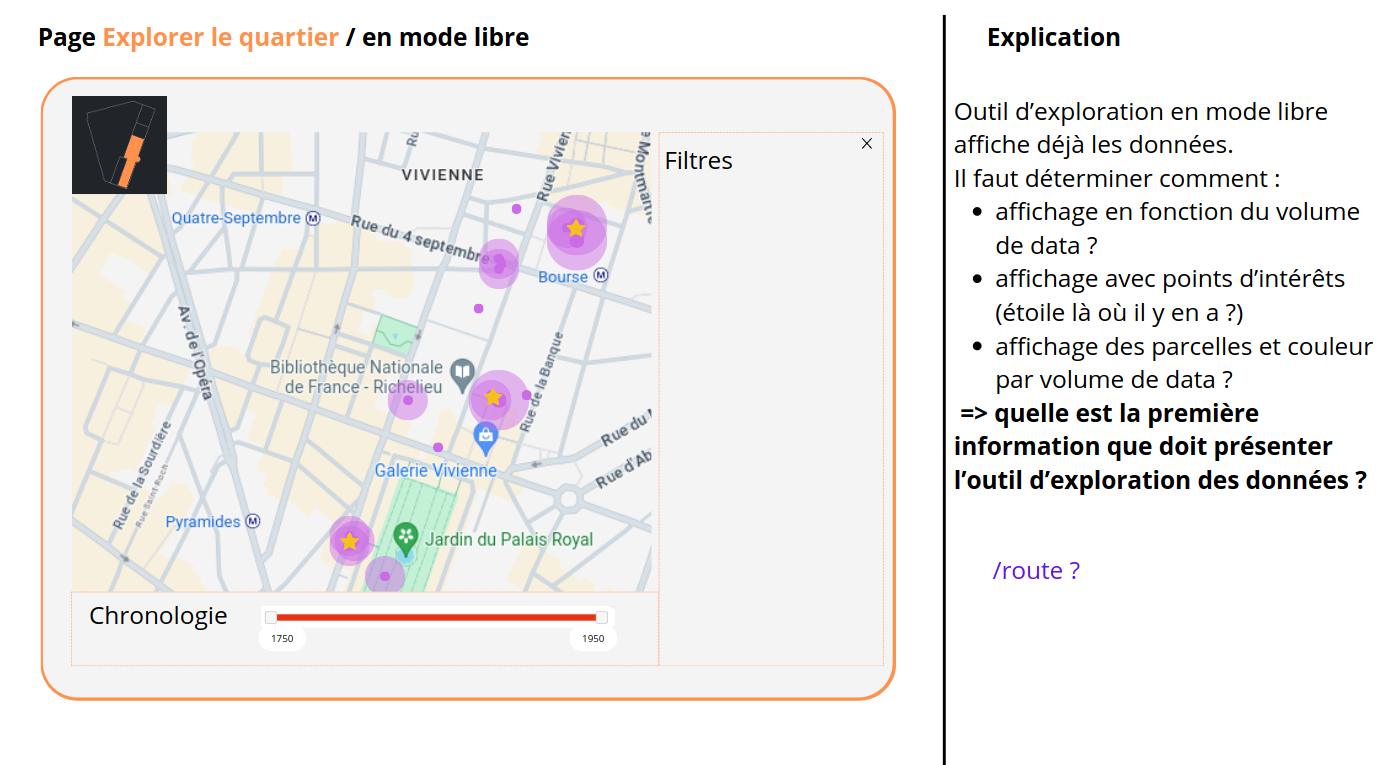
\includegraphics[width=1\linewidth]{images/storyboard-all.png}
    \caption{Storyboard page générale sur la carte}
    \label{fig:story-all}
\end{figure}
\subsubsection{Scénariser l'exploration}
Le premier objet du \textit{Storyboard} a été de scénariser l'arrivée de l'utilisateur sur la carte et de proposer une aide à sa prise en main. Ainsi un onglet \enquote{à propos} est pensé au même titre que ceux que nous avons cités et comparés dans les cartes plus-haut (voir la figure \ref{fig:story-propos}). Une particularité de cette page d'accueil est de proposer une exploration guidée. Si l'utilisateur choisit ce mode d'exploration alors les données affichées sur la carte sont pré-sélectionnées par les chercheurs de l'équipe en fonction d'un sujet pré-défini. Mais l'utilisateur peut également refuser cette proposition guidée pour explorer librement la carte. À partir de ces deux modes, les éléments structurels sont identiques.

\begin{figure}[h!]
    \centering
    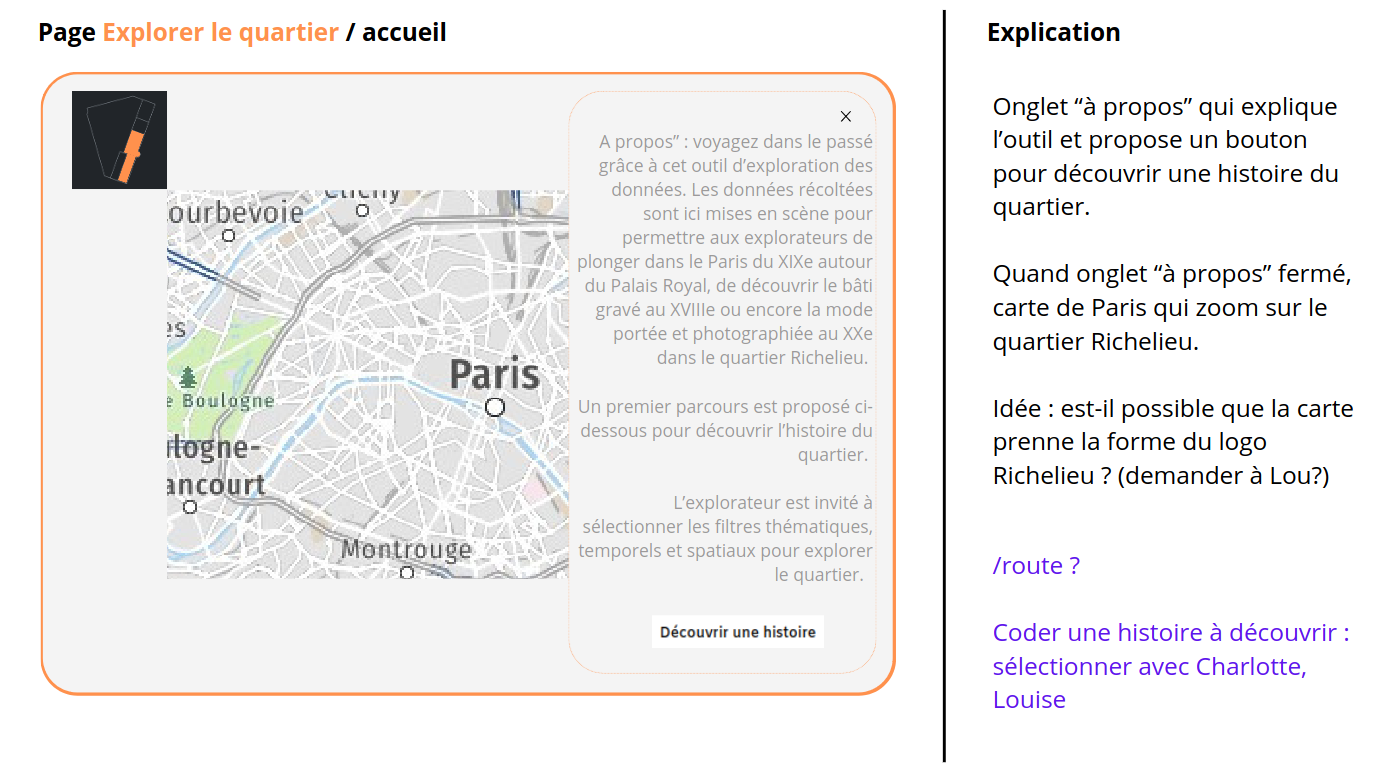
\includegraphics[width=1\linewidth]{images/storyboard-apropos.png}
    \caption{Storyboard page \enquote{à propos}}
    \label{fig:story-propos}
\end{figure}

\subsubsection{Le temps : la chronologie}\label{sous-sous-section:chrono}
Le temps est une notion intrinsèque au projet Richelieu. Sa représentation graphique prend plusieurs formes dont la première, plus conventionnelle, est une frise chronologique. Partant de 1750 pour s'étendre jusqu'à 1950, elle est liée à tous les documents datés. Plusieurs niveaux de détail peuvent s'ajouter à cette frise. Le premier niveau consiste à choisir une date au sein de cette période. Le curseur placé sur 1834, par exemple, affichera toutes les données qui sont précisément liées à cette date. Toutes les autres données sont exclues et n'apparaissent pas sur la carte. Le deuxième niveau proposé consiste à choisir une période au sein de la frise. Seules les données de la période sélectionnées entre deux curseurs sont affichées, le reste est également exclu. Enfin, le troisième niveau plus complexe à conceptualiser propose une sélection plus détaillée. Ce niveau permet de choisir une période et une date précise au sein de celle-ci. La visualisation graphique des données mettrait en exergue cette distinction (comme le propose la figure \ref{fig:story-chrono}). 
Lors des échanges sur la frise chronologique, des questions émergent. Les chercheurs savent que les données ne s'étalent pas de façon homogène sur toute la période. Certaines dates sélectionnées afficheront un très grand nombre de données et elles risquent d'être écrasées par leur volume. On se demande alors s'il faut distordre la frise chronologique et visuellement signifier cette volumétrie occupée par les données. C'est un point soulevé très intéressant à retenir pour des développements futurs.

\begin{figure}[h!]
    \centering
    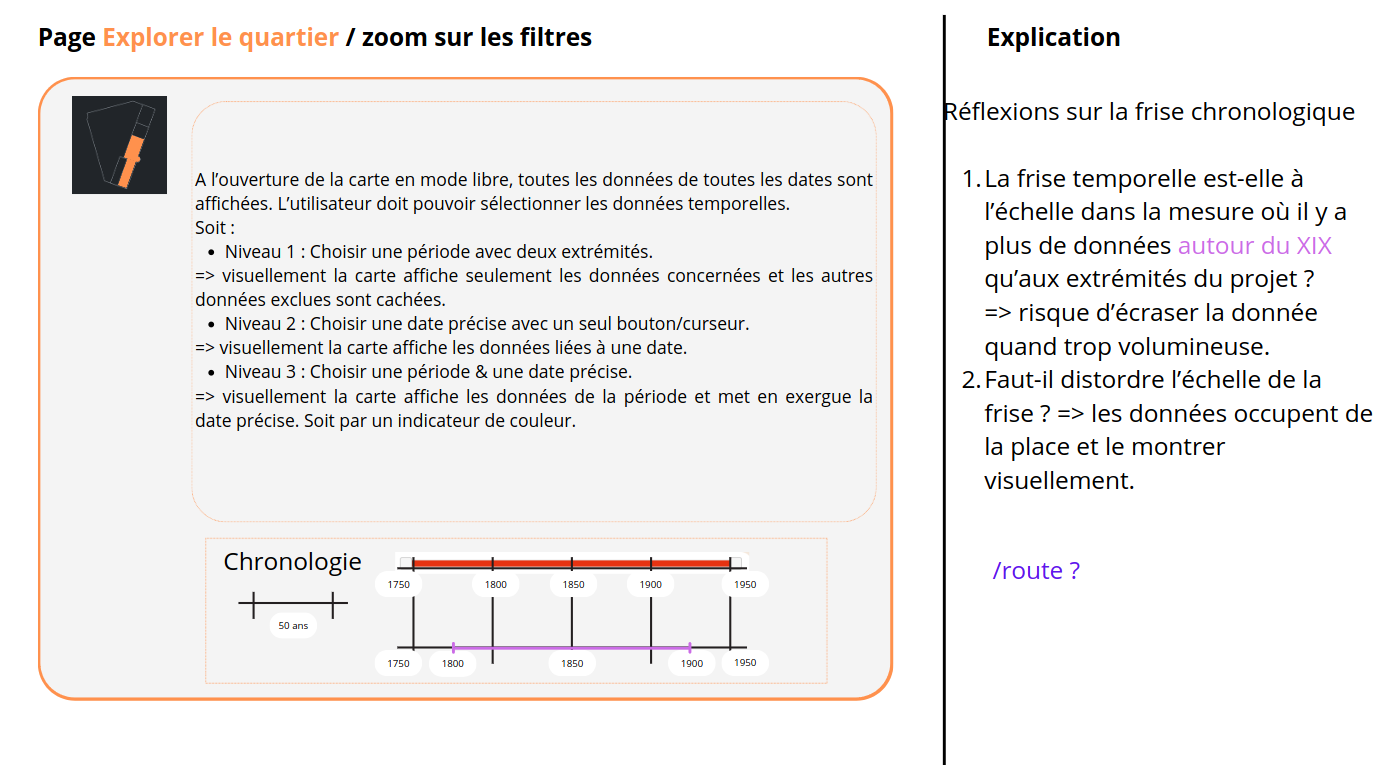
\includegraphics[width=1\linewidth]{images/storyboard-chrono.png}
    \caption{Storyboard page \enquote{chronologie}}
    \label{fig:story-chrono}
\end{figure}

\subsubsection{L'espace : les filtres}
Pour représenter la notion spatiale dans le projet Richelieu, une proposition est de laisser à l'utilisateur la possibilité de choisir le niveau de granularité des données. Nous avons vu que les sources cartographiques sont définies par leur niveau de granularité, parmi lesquels : l'aile, la galerie, l'ensemble et la parcelle. Grâce à un système de filtre à cocher, l'utilisateur peut sélectionner le niveau qu'il souhaite afficher. Ces filtres ont aussi pour objectifs additionnels, combinés entre-eux : c'est-à-dire que tous les niveaux peuvent être affichés, ou seulement un seul ou certains d'entre eux. Ce niveau de granularité ne se mettrait pas à jour en fonction du niveau du zoom car l'échelle du quartier est déjà suffisamment réduite. Cette fonctionnalité a pour but de montrer à l'utilisateur l'évolution parcellaire.

\subsubsection{La double dimension spatio-temporelle : les filtres par fond de carte historique}

L'espace et le temps sont deux dimensions qui, lorsqu'elles sont reliées à la carte, représentent une double dimension spatio-temporelle : l'idée de la spatialisation du temps et de la temporalisation de l'espace. En se faisant se succéder plusieurs cartes historiques, on peut remarquer l'évolution bâtie que ce soit par la construction de nouveaux bâtiments ou par l'ouverture de nouvelles rues. Pour ce faire, nous proposons des filtres à cocher par fond de carte historiques. L'utilisateur pourra, au même titre que les filtres de granularité, sélectionner un ou plusieurs filtres. 

\subsubsection{La sémantique : les filtres thématiques}

Afin de structurer la donnée, nous avons vu que l'équipe réunit les sources documentaires en six grands thèmes: \enquote{Se divertir}, \enquote{Habiter}, \enquote{Consommer}, \enquote{S'habiller}, \enquote{Représenter}, \enquote{S'informer}. Chacun réunit des sous-thèmes appelés \textbf{entités nommées} dans la base de données. L'idée est ainsi de représenter le quartier à travers plusieurs notions sémantiques, que nous envisageons comme autant de filtres thématiques encapsulant les entités nommées regroupées par thèmes. Pour leur visualisation, nous verrons s'ils sont repérés à l'aide de pictogrammes ou plutôt via un système de couleurs.

\begin{figure}[h!]
    \centering
    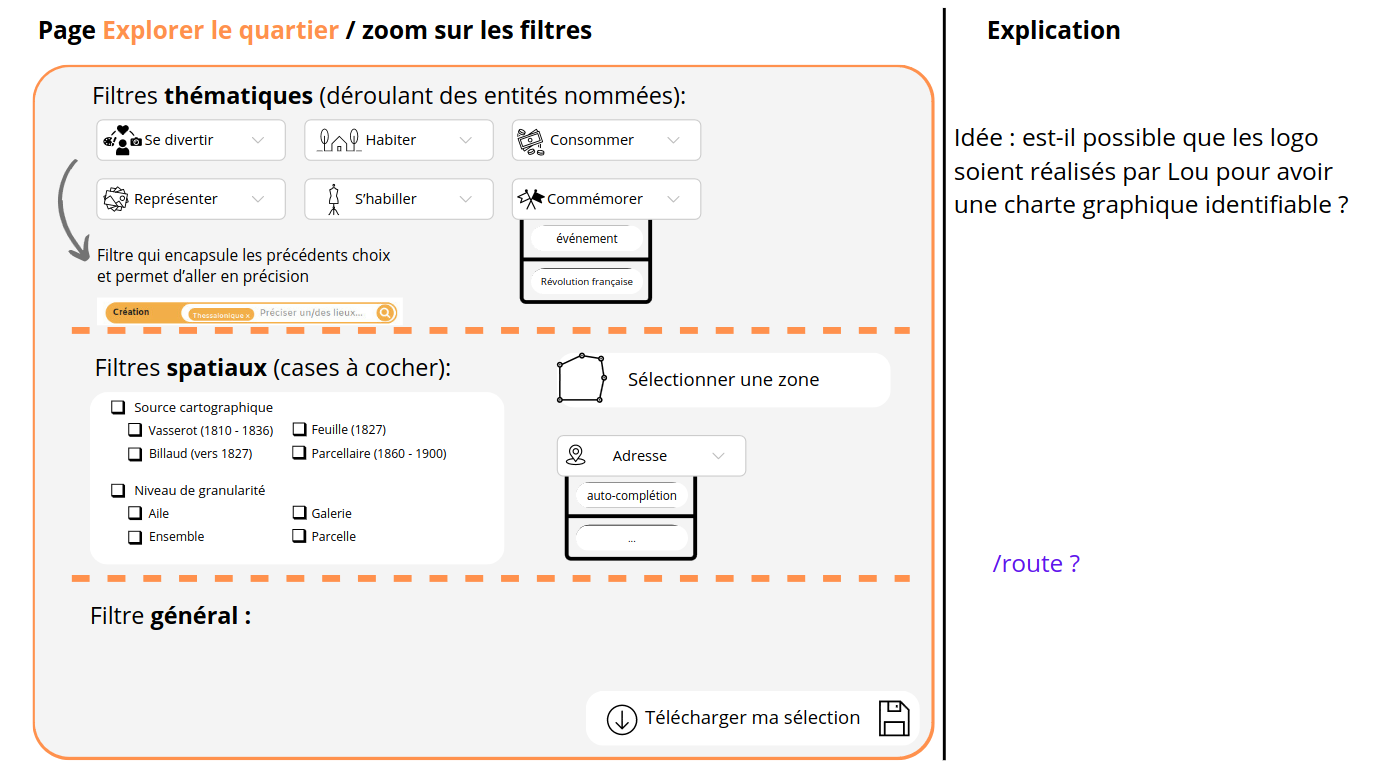
\includegraphics[width=1\linewidth]{images/storyboard-filtres.png}
    \caption{Storyboard page \enquote{filtres}}
    \label{fig:story-filtres}
\end{figure}

\subsubsection{L’iconographie : le carrousel d’images}

Pour représenter l'iconographie, la méthode la plus directe consiste à afficher les images provenant des sources iconographiques. Chaque parcelle étant associée à un ensemble d'iconographies, il est envisagé qu'un carrousel d'images s'affiche lorsqu'un lieu est cliqué sur la carte par l'utilisateur. Toutefois, il existe un risque de saturation de l'espace de visualisation lorsque le nombre d'images liées à un lieu est trop important, certaines images seraient alors inaccessibles car noyées dans une trop large sélection. Les filtres jouent un rôle crucial pour atténuer ce problème. En effet, les iconographies sont accompagnées de métadonnées structurelles et descriptives, qui peuvent être utilisées comme filtres, tels que les thèmes, les dates et les sources cartographiques associées.

La combinaison de l'ensemble de ces filtres permet à l'utilisateur d'afficher les données avec précision. Telle est l'interaction conceptualisée pour la carte. 

\subsubsection{D'autres possibilités}
Toutefois, d'autres possibilités de navigation sont émises lors de réunions de travail. 
\textbf{La barre de recherche} permet de saisir un champ au sein de la carte, telle qu'une adresse, pour afficher instantanément les informations qui y sont liées. Même si cette barre est couramment utilisée sur les sites Web, son développement est particulièrement difficile à mettre en place. Toutefois, elle offre quelques avantages comme l'accès rapide aux données. \textbf{La sélection de zone personnalisée} est une fonctionnalité conçue pour évoquer l'utilisation d'une carte papier, retournée et orientée selon la direction de marche, où les utilisateurs entourent, annotent et crayonnent ce qui les intéresse. Pour reproduire cette matérialité, l'idée est de permettre à l'utilisateur d'interagir directement avec la carte. Les données affichées sont alors exclusivement liées à la zone qu'il a dessinée. Cette fonctionnalité est particulièrement utile pour un chercheur qui, par exemple, se concentre sur un bâtiment spécifique et souhaite accéder uniquement aux informations le concernant. Enfin, la possibilité de \textbf{télécharger les données sélectionnées} depuis une carte permet à l'utilisateur de conserver et d'analyser ces informations en dehors de l'interface initiale. Cela facilite leur utilisation pour des recherches ultérieures. Pour un chercheur, par exemple, cela offre l'avantage de pouvoir manipuler plus en précision les données avec des logiciels spécialisés, favorisant ainsi des analyses plus approfondies que celles permises par la carte. Cette extraction en fonction des besoins spécifiques participe aussi au partage des données. 

\subsubsection{\textit{Quid} du réseau ?}
Les réflexions menées au cours du stage montrent que la notion de « réseau » ne sera pas explicitement représentée sur la carte. Le lieu, en tant qu'entité centrale du projet, est considéré comme la manifestation du réseau, car toutes les informations y sont reliées par la base de données relationnelle. Bien que l'idée d'accompagner la carte d'une visualisation en réseau ait été envisagée, il aurait été nécessaire de déterminer sa pertinence, en se demandant si elle sert à démontrer un propos ou si elle s'inscrit dans une démarche de recherche, selon les distinctions faites par Grandjean.
\\

Les fonctionnalités sus-mentionnées offrent aux utilisateurs, qu'ils soient chercheurs ou novices, une expérience personnalisée et précise. Ces outils ont pour objectif d'offrir une meilleure compréhension du quartier étudié, mais aussi une exploitation approfondie des données. Il convient de rappeler qu'il ne s'agit ici que d'une conceptualisation, définissant des possibilités dont la faisabilité ne sera confirmée qu'au cours du développement informatique. Seule la mise en production permet en effet de déterminer si ces idées peuvent être concrètement réalisées. 

\subsection{Le \textit{MVP} : hiérarchiser les priorités}
Le \textit{Minimum Viable Product}, largement utilisé dans le développement de produits, notamment dans le secteur des technologies, consiste à créer une version simple, basique et fonctionnelle d'un produit, en l'occurrence d'une carte. Après avoir listé les fonctionnalités d'un produit, le  \acrshort{mvp} permet de les hiérarchiser selon un ordre de priorité de développement et d'évaluer la difficulté de leur mise en œuvre pour les développeurs, tout en s'assurant que le produit réponde aux besoins essentiels dès ses premières itérations. L'objectif principal de cette approche est de lancer rapidement un produit fonctionnel pour recueillir des retours d'expérience concrets, afin de vérifier son adéquation avec les attentes des utilisateurs. 

Pour le développement de la carte dans le cadre du projet Richelieu, un  \acrshort{mvp} (voir \ref{fig:mvp}) a été adopté pour clarifier les fonctionnalités, les structurer dans le temps, et garantir une progression méthodique vers la version finale de la géodatavisualisation. Cette approche permet non seulement de tester la carte dès les premières phases de son développement, mais aussi d'affiner ses fonctionnalités en fonction des retours, tout en respectant les contraintes du projet. Le  \acrshort{mvp} sert ainsi de feuille de route, permettant de suivre l'avancement du développement à chaque étape. Les fonctionnalités en orange sont considérées comme réalisables avec un effort minimal et un faible impact pour le projet final. Elles seront probablement développées en priorité dans les premières étapes du projet informatique. Les fonctionnalités en vert sont les éléments essentiels, les \textit{must have} du projet, dont la réalisation a un impact fort et demande un effort de développement acceptable. En rouge sont indiquées les fonctionnalités hors de notre portée de réalisation, telle que la version multilingue. Enfin, en bleu sont les fonctionnalités supplémentaires mais non essentielles au projet, incluant la sélection de zones personnalisées, le téléchargement des données sélectionnées et le parcours guidé. 

\begin{figure}[h!]
    \centering
    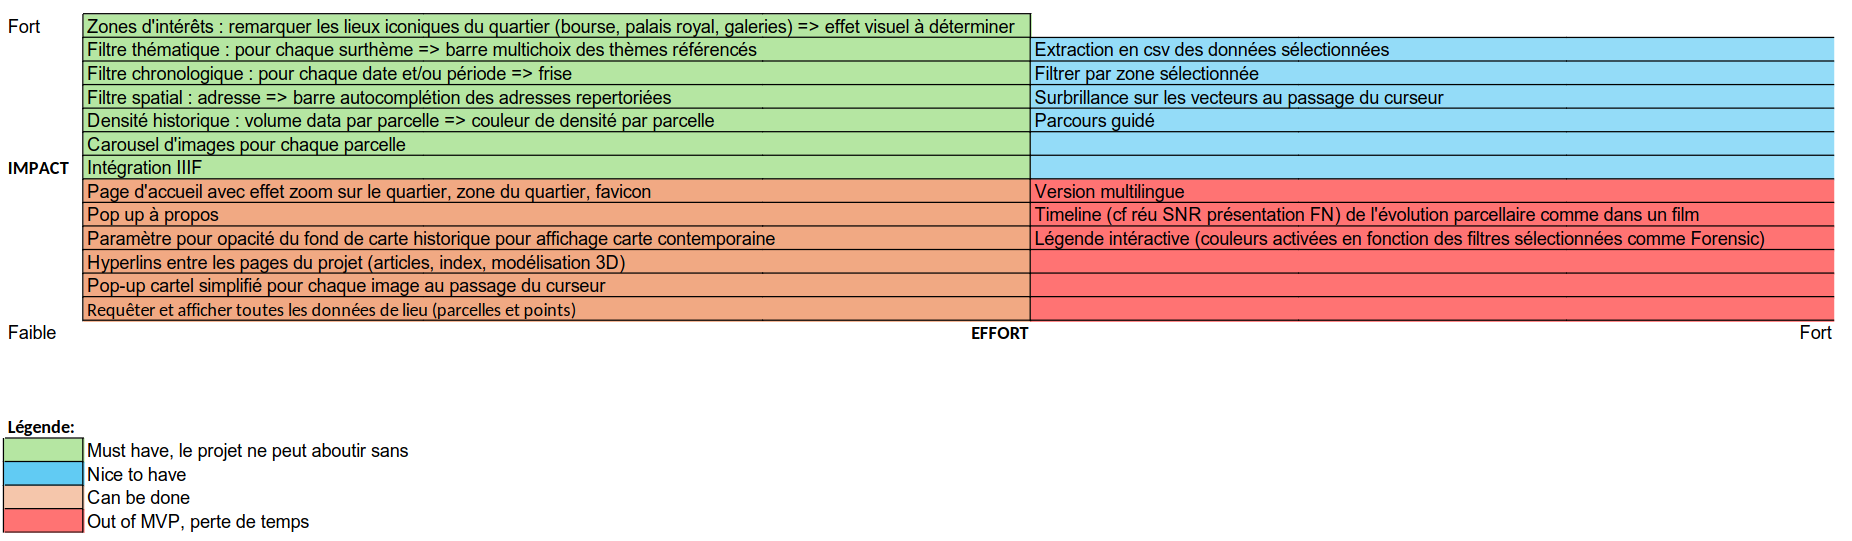
\includegraphics[width=1\linewidth]{images/MVP.png}
    \caption{ \acrshort{mvp} du projet Richelieu}
    \label{fig:mvp}
\end{figure}

Grâce au  \acrshort{mvp} et au \textit{Storyboard}, à considérer comme des outils de gestion du temps, notre feuille de route de développement s'est précisée et il convient de l'exécuter méthodiquement. 

%%%%%%%%%%%%%%%%%%%%%%%%%%%%%%%%%%%%%
% SECTION %%%%%%%%%%%%%%%%%%%%%%%%%%%
\section{Analyser la matérialité de la donnée contre l'effet « boîte noire ».}
La partie précédente du mémoire a exposé la structure de la base de données du projet Richelieu, nous permettant de comprendre comment les corpus sont transformés en données. Dans le chapitre actuel, nous avons également précisé la manière dont nous souhaitons représenter ces données sur la carte. En d'autres termes, nous avons une vision claire des données en entrée et de leur représentation en sortie. Cependant, avons-nous une \textit{overview} sur le contenu de la base de données dans toute sa complexité ? La visualisation graphique que nous observerons sur la carte est-elle réellement fidèle au contenu de la base ? Par exemple, si la carte indique qu'une parcelle est associée à 1000 images, comment savoir s'il s'agit d'une aberration ou d'un résultat authentique ? Jusqu'à quel point pouvons-nous faire confiance aux données visualisées ?  Est-ce que les données affichées sur la carte ont un sens ? Dans quelle mesure la carte invisibilise un récit sur le quartier et inversement ? 

Une analyse en profondeur de la matérialité des données évite l'effet \enquote{boîte noire} et permet de connaître leur volume, leur contenu et leurs particularités. Ce besoin est d'autant plus vrai lorsque l'ingénieur n'a pas conçu la base de données mais qu'il doit interagir et produire à partir de celle-ci. Pour cette étape, il s'agit de rendre visible ce qui est opaque. Ce travail est une précaution, permettant de savoir si la carte reflète les données de manière aussi précise et transparente que possible, minimisant ainsi les risques de biais ou d'erreurs dans la visualisation.

Pour ce faire, il s'agit ici de présenter une analyse comparative et quantitative des données. La base de données est interrogée grâce à un ensemble de requêtes  \acrshort{sql} générées sur pgAdmin\footnote{Voir annexes \ref{chapter:sql}} qui propose également un \textit{plugin} pour visualiser graphiquement les résultats. Les requêtes ne sont pas réalisées par corpus documentaire mais par dimension et point d'accès à la donnée sur la carte : le lieu, les sources documentaires et le temps. 

\subsection{Le lieu}\label{sous-section:lieu}
Nous avons montré que le lieu est l'entité centrale du projet. Toute information est donc reliée à un lieu, voire un groupe de lieux, sinon un document iconographique ou cartographique alors par la suite relié au lieu. 

\subsubsection{La répartition des sources par lieu}\label{sous-sous-section:rm19}

\begin{figure}[!]
    \centering
    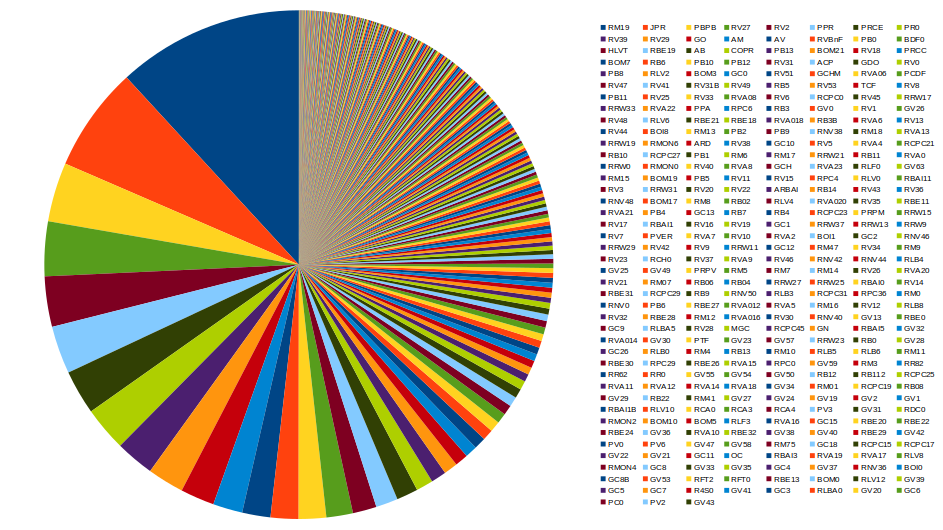
\includegraphics[width=1\linewidth]{images/graphiques/total_sources_lieu.png}
    \caption{La répartition totale des sources par lieu}
    \label{fig:répartition_totale_sources_lieu}
\end{figure}

La légende de ce graphique en camembert (figure \ref{fig:répartition_totale_sources_lieu}) est difficile à lire à cette échelle, il faut simplement retenir que chaque ligne de couleur représente un lieu différent. Le total des sources cartographiques par lieu a été calculé et additionné au nombre total de sources iconographiques par lieu pour donner un nombre total de sources par lieu. Celui-ci est représenté par le volume occupé par chaque part de couleur dans le graphique. On constate distinctement que la répartition du nombre de sources par lieu est loin d'être homogène. En effet, la moitié des sources se concentre sur seulement 14 des 331 lieux répertoriés par le projet. Autrement dit, 50\% des sources sont concentrées sur seulement 4,2\% des lieux, dont un quart seulement est associé à 4 lieux. Plus précisément, un lieu saute aux yeux, il s'agit de la part en bleu marine, le \enquote{RM19}, situé au 19, rue Montpensier et associé au Théâtre du Palais Royal (dont l'adresse a évolué au fil du temps). Il répertorie à lui seul 877 documents. Lieu emblématique de la culture parisienne, il est aussi producteur d'une abondante documentation liée au théâtre, notamment des affiches et des recueils de costumes d'acteurs et actrices, chaque recueil comptant en moyenne 200 pages. Par ailleurs, force est de constater que l'autre moitié des sources est répartie sur les 317 lieux restants, mais cette répartition est également inégale, comme le montre le graphique en barres suivant.

\subsubsection{La répartition des sources iconographiques (> 100) par lieu}
\begin{figure}[ht!]
    \centering
    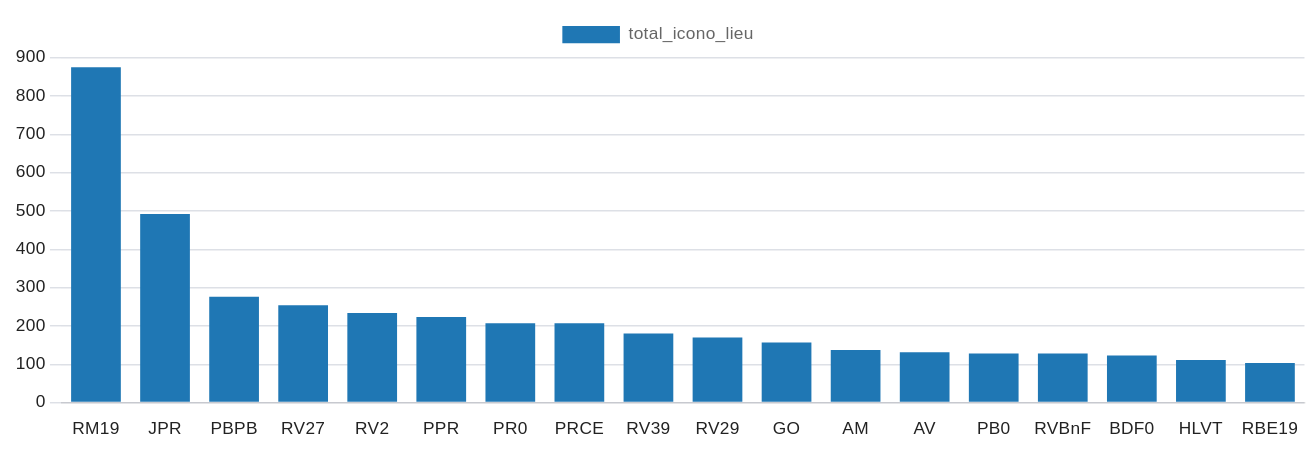
\includegraphics[width=1\linewidth]{images/graphiques/nb_icono_lieu_>100.png}
    \caption{Nombre d'iconographie par lieu (au moins 100)}
    \label{fig:répartition_totale_icono_lieu}
\end{figure}
Ce graphique (\ref{fig:répartition_totale_icono_lieu}) indique par ordre décroissant les lieux ayant plus de 100 sources iconographiques répertoriées.  À la lecture des lieux, on observe une représentation majoritaire de certaines zones géographiques. Les termes \enquote{JPR}, \enquote{PPR}, \enquote{PR0} et \enquote{PRCE} se rapportent tous au Palais Royal, que ce soit à son jardin, à l'ensemble architectural, à la place ou encore au Conseil d'État. De même, \enquote{PBPB} et \enquote{PB0} désignent la Place de la Bourse et le Palais Brongniart. Enfin, \enquote{RV} fait référence à la rue Vivienne. Ces trois lieux apparaissent clairement comme des points d'intérêt largement documentés dans le corpus iconographique, avec la rue Vivienne formant un axe central menant aux deux palais. Notons que les échelles de ces lieux sont différentes : certains sont des bâtiments, tandis que d'autres sont des ensembles viaires ou architecturaux. Or la question se pose de savoir comment éviter d'écraser les données lors de leur visualisation tout en respectant ces différentes échelles de représentations.

\subsubsection{Le nombre de sources cartographiques par lieu}
En ce qui concerne la répartition du nombre de sources cartographiques par lieu, une représentation dans un graphique en barre (\ref{fig:répartition_totale_carto_lieu}) est peu pertinent. On constate simplement que tous les lieux ont au moins une source cartographique. Pour comprendre combien de lieux sont référencés à une ou plusieurs sources cartographiques, le graphe en camembert ci-dessous (\ref{fig:repartition_carto_lieu}) donne à constater que 193 lieux sont référencés à une seule source cartographique, 113 en ont 2, 24 en ont 3 et seulement un lieu, le 17, rue Vivienne (\enquote{RV17}) est référencé dans les 4 sources cartographiques géoréférencées du projet. Très peu de lieux ont une couverture cartographique dense. Cela suggère une documentation partielle de l'évolution parcellaire, probablement liée à la stabilité de certains lieux, comme indiqué dans la méthode régressive évoquée précédemment (\ref{par:méthodes}).

\begin{figure}[ht!]
    \centering
    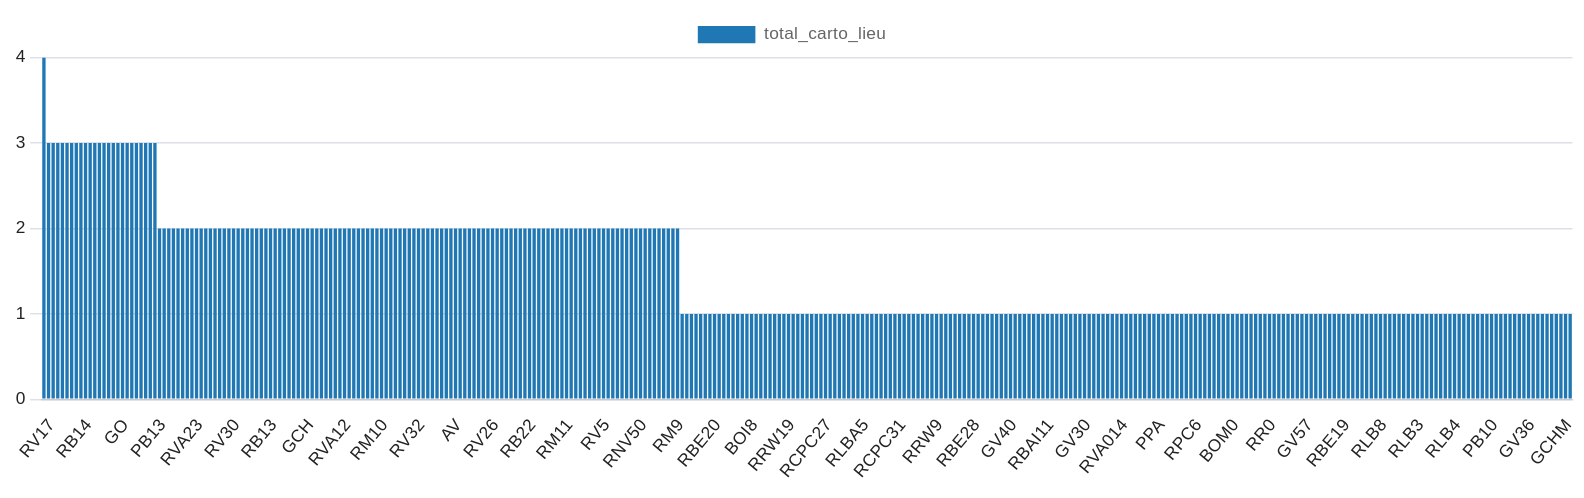
\includegraphics[width=1\linewidth]{images/graphiques/nb_carto_lieu_barChart.png}
    \caption{Nombre de cartographies par lieu}
    \label{fig:répartition_totale_carto_lieu}
\end{figure}

\begin{figure}[ht!]
    \centering
    
\includegraphics[width=0.8\linewidth]{images/graphiques/repartition_lieux_nb_carto_lieu_pie.png}
    \caption{Répartition totale des lieux par source cartographique par lieu.}
    \label{fig:repartition_carto_lieu}
\end{figure}

En résumé, cette première analyse met en évidence une concentration marquée des sources iconographiques et cartographiques sur un nombre restreint de lieux, avec une répartition inégale. Bien que certains affichages nous apparaissent comme aberrants, il convient d'indiquer que certains types de graphiques illustrent mieux les données que d'autres. En réalité, il s'agit d'une distribution déséquilibrée des sources par lieu.  Cette observation est essentielle à garder à l'esprit lors du développement afin d'éviter toute distorsion des données et de garantir une représentation fidèle et équilibrée du patrimoine étudié.

\subsection{Les corpus documentaires}
Les corpus documentaires du projet sont aussi un point d'entrée dans l'application. Intéressons-nous à la provenance de la majorité des sources et aux principaux médiums 

\subsubsection{La répartition des sources par institution}
Identifier les principales sources du projet Richelieu, c'est-à-dire les lieux de conservation des documents iconographiques et cartographiques, permet d'évaluer si la base de données reflète véritablement les ambitions initiales du projet. L'analyse révèle que les sources proviennent de 26 institutions différentes, mais près de 83\% d'entre elles sont concentrées dans seulement quatre institutions : le Musée Carnavalet (1333 sources), la \acrshort{bnf} (1312 sources), les bibliothèques spécialisées de la ville de Paris (928 sources), et la Bibliothèque historique de la ville de Paris (827 sources). Quant aux sources cartographiques, elles sont principalement issues de centres d'archives. 
\begin{figure}[ht!]
    \centering
    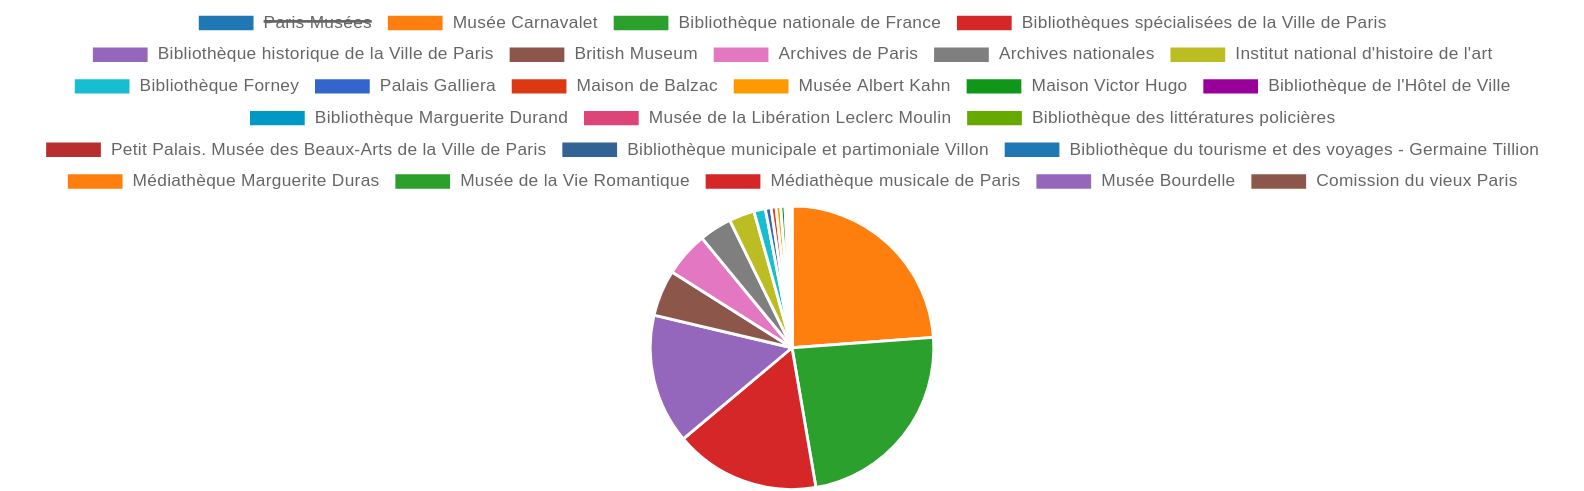
\includegraphics[width=1\linewidth]{images/graphiques/total_sources_institution.png}
    \caption{Nombre de sources par institution (1/2)}
    \label{fig:sources_institution}
\end{figure}
\begin{figure}[ht!]
    \centering
    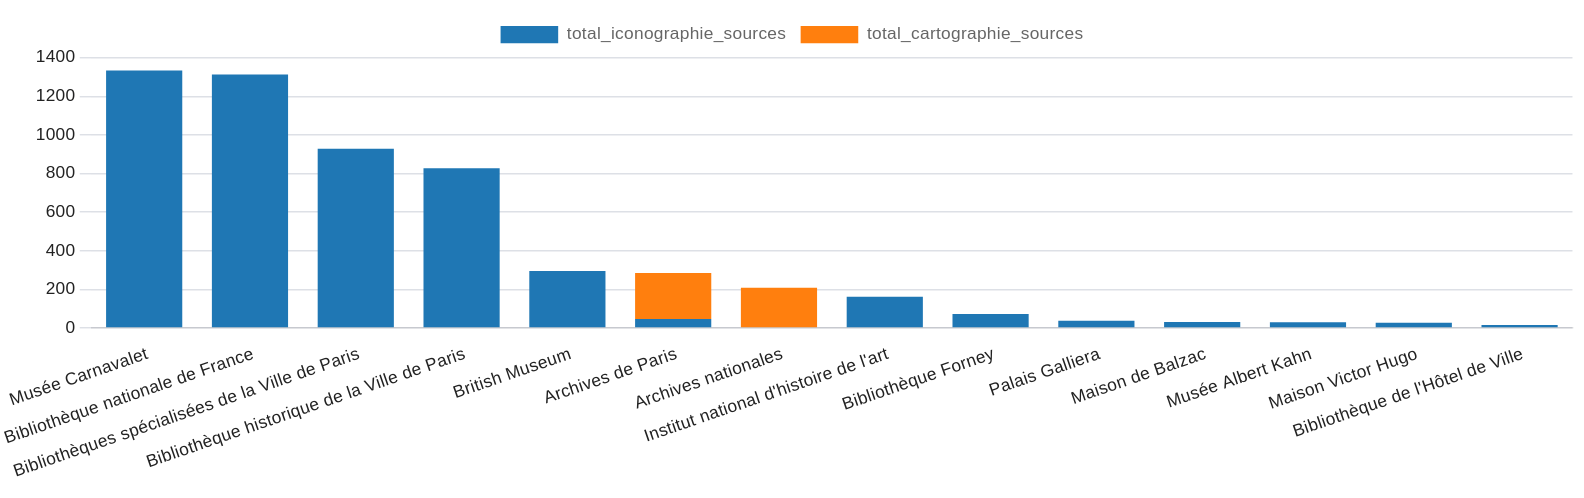
\includegraphics[width=1\linewidth]{images/graphiques/total_source_institution.png}
    \caption{Nombre de sources par institution (2/2)}
    \label{fig:sources_institution2}
\end{figure}
Ainsi, la majorité des données historiques du projet ne proviennent pas des principaux acteurs, à l'exception notable de la \acrshort{bnf}. Pourtant, l'une des motivations premières du projet était de découvrir l'histoire à travers les collections de ces institutions, elles-mêmes porteuses du projet. Il se pourrait que ce résultat soit influencé par les politiques de numérisation variables selon les institutions ou par le lien spécifique des collections avec le quartier concerné.

\subsubsection{La répartition des iconographies par medium}
Identifier la répartition des médiums au sein du corpus iconographique donne à voir d'autres caractéristiques du corpus.

\begin{figure}[ht!]
    \centering
    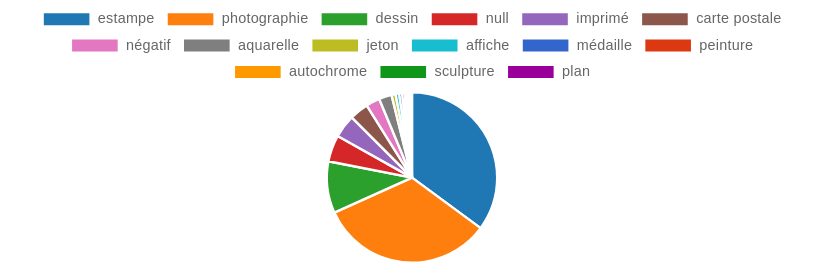
\includegraphics[width=1\linewidth]{images/graphiques/nb_icono_technique>10.png}
    \caption{Répartition des iconographies par technique}
    \label{fig:icono_technique}
\end{figure}

On constate que la majorité des documents iconographiques rassemblés dans le projet sont des estampes et des photographies, deux médiums qui ont joué un rôle central dans la représentation visuelle au XIX\ieme~ siècle et au XX\ieme~ siècle respectivement. Cette prédominance s'explique non seulement par leur importance historique, mais aussi par les choix de numérisation effectués par les institutions patrimoniales. En effet, la numérisation d'estampes et de photographies est techniquement plus simple et moins coûteuse que celle d'œuvres d'art plus fragiles comme les peintures, les sculptures ou les autochromes, qui nécessitent des techniques de capture plus sophistiquées et des traitements spécifiques. Par conséquent, la composition de cette collection numérisée reflète à la fois les priorités historiques et les contraintes techniques des institutions en matière de conservation numérique.

\subsection{Le temps}
Pour le projet Richelieu, le temps est une dimension à faire figurer dans la visualisation des données historiques. Dans le cadre d'un projet visant à explorer des périodes historiques, à remonter dans le temps en somme, il est essentiel d'examiner attentivement la répartition temporelle des sources disponibles.

\subsubsection{La répartition temporelle des sources : par intervalle de 50 ans}
Ce graphique (\ref{fig:total_sources_date50}) met en évidence une répartition inégale des sources selon des intervalles de 50 ans. Le XIX\ieme~ siècle est largement représenté avec un nombre significatif de sources, en particulier durant la seconde moitié du siècle. En revanche, le XX\ieme~ siècle et le XVIIIe siècle sont moins bien représentés en termes de volume de sources. Cette disparité s'explique probablement par plusieurs facteurs qui échappent à la sélection intentionnelle des chercheurs. Le XIX\ieme~ siècle a vu une intensification de la production d'informations, notamment grâce aux progrès des techniques de reproduction initiés par la révolution industrielle, qui ont également favorisé l'essor du journalisme et de la photographie. À l'inverse, le XVIIIe siècle est moins représenté, car les techniques de reproduction de l'époque étaient principalement artisanales, et non industrielles, ce qui a limité la production et la préservation des documents. Pourtant, on pourrait hâtivement penser que les sources deviennent plus abondantes avec l'avancée du temps, et le développement des techniques de reproduction de l'information ainsi que celles de conservation.
\begin{figure}[ht!]
    \centering
    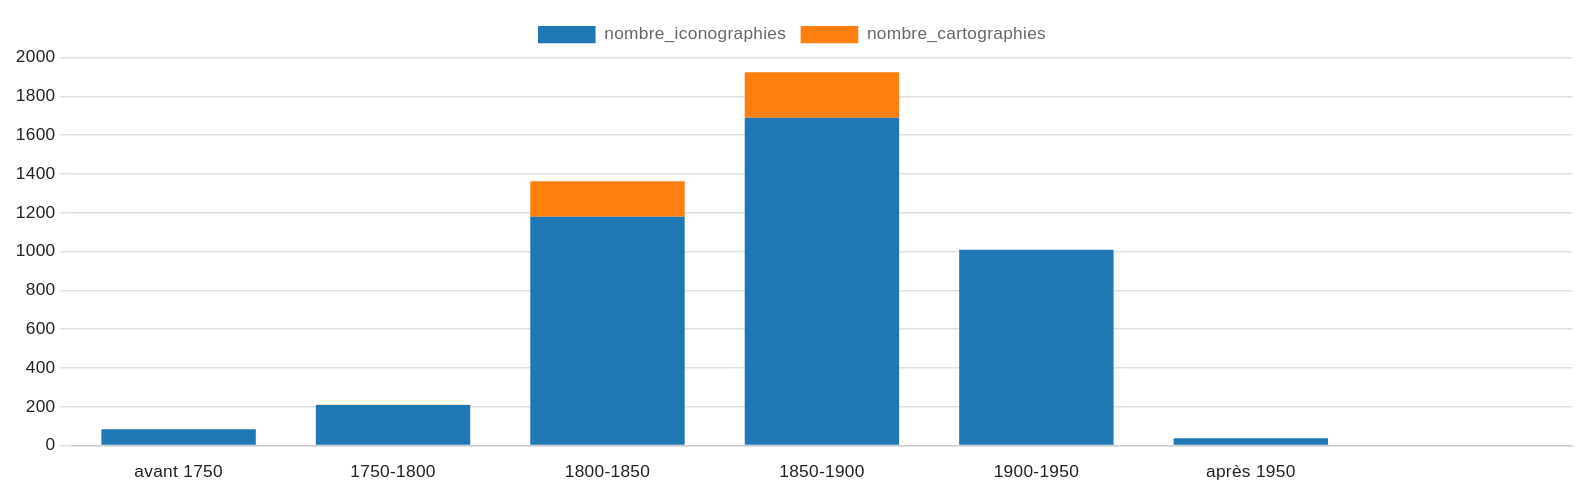
\includegraphics[width=1\linewidth]{images/graphiques/total_source_date_50.png}
    \caption{Nombre total de sources par date (intervalle de 50 ans)}
    \label{fig:total_sources_date50}
\end{figure}
Un point surprenant soulevé par le graphique est la présence de documents qui dépassent les bornes chronologiques initialement définies pour le projet. On trouve en effet une petite proportion de documents datant d'avant 1750 et d'après 1950. Cette anomalie soulève des questions quant à la pertinence de leur inclusion. Il serait intéressant de demander aux chercheurs de justifier leur présence et de déterminer si leur intégration dans la frise chronologique est vraiment nécessaire ou si ces documents pourraient être retirés pour mieux respecter les bornes temporelles du projet.

\subsubsection{La répartition temporelle des sources : par intervalle de 10 ans}
\begin{figure}[ht!]
    \centering
    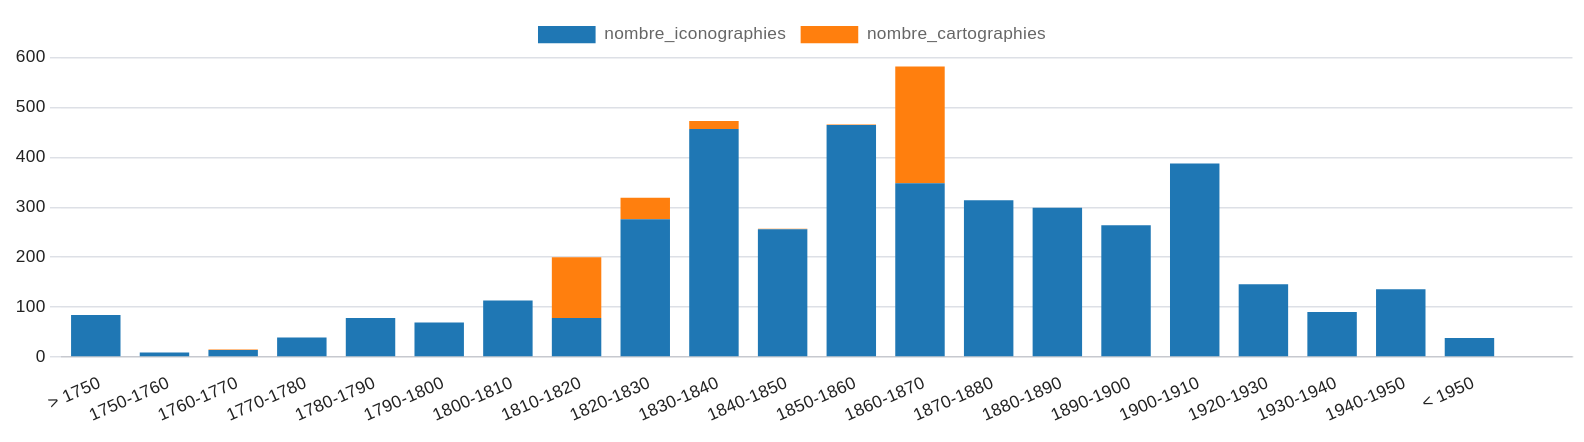
\includegraphics[width=1\linewidth]{images/graphiques/total_source_date_10.png}
    \caption{Nombre total de sources par date (intervalle de 10 ans)}
    \label{fig:total_sources_date10}
\end{figure}
L'analyse à une échelle plus fine permet de révéler des nuances importantes dans la répartition des sources. Par exemple, il est particulièrement surprenant de constater que le nombre de sources datant d'avant 1750 dépasse celui des sources comprises entre 1750 et 1780. Ces sources antérieures pourraient ainsi compenser le déficit observé pour certaines périodes couvertes par le projet. De manière générale, on observe une concentration des sources sur un XIX\ieme~ siècle élargi, qui commence avec la Révolution française et s'étend jusqu'à la veille de la Première Guerre mondiale.

Cependant, une telle visualisation des données présente certains biais interprétatifs. Elle pourrait induire en erreur en suggérant que le projet adopte une approche historiographique particulière, alors même que ce postulat n'a pas été explicitement formulé au début des études sur le quartier Richelieu. De plus, cette visualisation peut donner l'impression que le projet présente des lacunes en sources cartographiques, notamment à partir de la seconde moitié du XIX\ieme~ siècle. Or, il est important de noter que les sources cartographiques sont souvent rattachées à des périodes spécifiques en fonction de la réalité bâtie, ce qui signifie qu'un bâtiment, une fois cartographié, peut ne pas nécessiter de nouvelles cartographies tant qu'il reste inchangé. Par exemple, un bâtiment construit en 1800 apparaîtra sur un plan de 1812 et pourrait rester inchangé jusqu'à aujourd'hui, mais sa présence dans la base de données sera seulement répertoriée dans l'intervalle 1810-1820, selon la date de création du dit plan. Enfin, le graphique omet de mentionner les données non datées, ou \enquote{NULL}, qui ne sont pas représentées ici. Le résultat de la requête \acrshort{sql} en donne pourtant 333, et leur exclusion pourrait également influencer la compréhension globale de la répartition des sources dans le projet.  

Cette étape de travail n'a pas pour objectif de mettre en lumière d'éventuelles lacunes du projet en termes de volume de données ou de répartition, mais plutôt de comprendre les raisons sous-jacentes et d'identifier des explications. Elle m'a permis de saisir comment la recherche a été menée, quels sont les principaux intérêts des chercheures et, surtout, comment la recherche a été traduite en données concrètes dans la base de données.

L'analyse du contenu de cette base résulte d'un travail long et manuel que j'ai personnellement accompli, mais la partie suivante permettra de souligner qu'une méthode de validation des données, qu'elle soit automatisée ou hybride, pourrait simplifier ce processus.

\subsection{Une méthode recommandée : mise en place de processus hybrides de validation}

Pour garantir la qualité et la fiabilité des données affichées, il est pertinent d'adopter des processus de validation combinant automatisation et intervention humaine, autrement dit, des méthodes hybrides. Cette approche permet d'allier l'efficacité des processus automatisés avec la précision et le discernement de l'analyse manuelle, assurant ainsi une validation plus rapide et plus fiable des données.

La mise en place de scripts de validation constitue un élément central de cette méthode. Ces scripts pourraient effectuer des contrôles systématiques, tels que la détection de valeurs manquantes, la vérification de la conformité des formats de données (comme les dates ou les coordonnées géographiques), et l'identification de doublons. Ils pourraient également évaluer la densité des données par catégorie, période ou lieu, ce qui permettrait de repérer les déséquilibres ou les lacunes susceptibles de biaiser les analyses, comme nous l'avons précédemment exposé. 

Toutefois, ces contrôles automatisés doivent être complétés par une validation manuelle qui interroge directement la base de données via l'interface graphique du  \acrshort{sgbdr} afin de garantir un contrôle robuste des données et d'offrir par ailleurs des indications précieuses aux utilisateurs. Par exemple, l'ajout d'indicateurs métriques sur la carte pourrait être envisagé. Ainsi, un chercheur serait informé si sa requête ne représente qu'un faible pourcentage du total des données, l'incitant éventuellement à élargir sa recherche. Bien que de tels indicateurs soient parfois mentionnés, l'ensemble de cette méthode de validation exige toutefois un investissement en temps supplémentaire. Cette méthode n'a pas pu être mise en œuvre pour le développement de la carte\footnote{Ce paragraphe est le fruit de discussions avec les membres du SNR, externes au projet, au cours du stage.}. Finalement, la méthode utilisée est une validation croisée qui consiste à comparer les données affichées sur la carte et celles requêtées directement en  \acrshort{sql} sur la base de données. 


Pour conclure, cette analyse approfondie du contenu de la base de données a permis de dégager les principales orientations du projet. Il en ressort que la majorité des documents sont des iconographies provenant du Musée Carnavalet et, plus largement, des collections de l'établissement Paris Musées, couvrant une période s'étendant de 1820 à 1870. Nous remarquons que le volume d'informations n'est pas uniformément réparti sur les deux siècles étudiés dans le cadre du projet. De plus, les différentes couches d'informations varient considérablement d'un lieu à un autre, certaines zones étant beaucoup plus riches en données que d'autres. Ces caractéristiques, tant temporelles que spatiales, ont des implications directes pour la mise en visualisation des données sur la carte. La concentration des sources dans certaines périodes ou dans des lieux spécifiques nécessite une attention particulière lors de la conception de la cartographie, afin de garantir une représentation équilibrée et fidèle des données. Il s'agit de se demander comment éviter de sur-représenter certaines périodes ou certains lieux, au détriment d'autres, et de veiller à ce que la carte reflète avec précision la réalité complexe et parfois déséquilibrée des sources historiques. 
Nous pensons que c'est en tenant compte de ces disparités que le potentiel exploratoire de la carte pourra pleinement s'exprimer. La carte ne se contentera pas d'être un simple outil de visualisation, mais elle dévoilera également les dynamiques historiques et spatiales sous-jacentes, permettant une interprétation plus riche et instructive des données. La carte serait \textit{démonstration} et \textit{recherche}. Cette approche transforme la carte en un instrument d'exploration du patrimoine étudié, en tenant compte  des spécificités et des biais propres à la base de données.

\subsubsection{Conclusion du chapitre}
Grâce à ce chapitre, nous avons vu que la définition des objectifs de développement spécifiques à la visualisation des données par cartographie Web est essentielle et antérieure à l'étape de développement. Elle permet notamment d'assurer la cohérence et l'orientation de la carte afin que celle-ci corresponde aux axes de recherche du projet. Cela permet de gagner en précision sur les fonctionnalités à développer, les données à intégrer, les choix techniques à privilégier. Les besoins des publics visés (novices ou experts) sont aussi à recueillir dans la mesure du possible. Cette étape permet aussi de comprendre le contexte de production des cartographies Web dans lequel le projet s'inscrit.
